\section{Extracting interval gluings from actual normal coordinates}
\label{sec:normal-interval-extraction}

The input to this section is a finite tetrahedral triangulation
$\mathcal T$ of a compact PL $3$-manifold, with $t$ tetrahedra, and an
admissible normal vector $x\in\mathbb N^{7t}$. The manifold hypothesis is
a mathematical precondition. The implemented extractor checks the face-pairing
schema, reciprocal identifications, nonnegative coordinates, quadrilateral
constraints, and matching equations; it does not check manifold links or a
conversion from a knot diagram. Orientability of the ambient manifold is not
needed for the extraction theorem.

Coordinates are ordered as
\[
 (T_0,T_1,T_2,T_3,Q_{01\mid23},Q_{02\mid13},Q_{03\mid12}).
\]
A quadrilateral $Q_{ab\mid cd}$ avoids the opposite edges $ab$ and $cd$.
We distinguish the side containing vertex $0$, denoted $A$, from its
complement $A^c$. Triangle discs at vertex $v$ are numbered from that vertex
outwards. Quadrilateral discs are numbered from the side $A$ towards $A^c$.
All indices and intervals in the implementation are zero-based and half-open.

\subsection{The face-order calculation}

Consider the face opposite vertex $f$ and an arc type cutting off vertex
$v\ne f$. There is a triangle block of size $T_v$. There may also be a
quadrilateral block: it is present exactly when the active quadrilateral
separates $\{f,v\}$ from the other two vertices. In the order from $v$
outwards, the triangle block precedes the quadrilateral block. If the latter
has size $Q$, its $j$th disc has face rank
\begin{equation}
 r(j)=
 \begin{cases}
  T_v+j,& f\in A,\\
  T_v+Q-1-j,& f\notin A.
 \end{cases}
 \label{eq:normal-face-rank}
\end{equation}
For triangles the face rank is simply $r(j)=j$.

This reversal is essential. One cannot number the quadrilateral stack
outwards from all four face vertices simultaneously. To see the geometry
directly, realize the quadrilateral discs by levels of
$\sum_{a\in A}z_a$ in barycentric coordinates. On a face missing a vertex of
$A$, this sum is the coordinate of the cut-off vertex; on a face missing a
vertex of $A^c$, the complementary sum is that coordinate. These orders
are opposite.

A simplicial face pairing sends the corner $v$ to its image corner and
preserves the normal arcs' rank from that corner. Suppose source and target
blocks use rank charts
\[
 r=\sigma i+\beta,\qquad r=\tau j+\gamma,
 \qquad \sigma,\tau\in\{1,-1\}.
\]
On the intersection of their rank intervals, their disc indices satisfy
\begin{equation}
 j=\tau\sigma i+\tau(\beta-\gamma).
 \label{eq:normal-face-pairing}
\end{equation}
Thus every nonempty block intersection produces an exact interval
translation or reflection, with no individual discs constructed.

\begin{theorem}[Linear normal-gluing extraction]
\label{thm:normal-five-bands}
From $(\mathcal T,x)$ one can construct a polygon-gluing presentation of the
represented normal surface using at most $5t$ nonempty polygon stacks and
at most five affine interval pairings per paired tetrahedral face. Polygon
templates specify the cyclic corner-edge labels, and every pairing retains
its source face, target face, and vertex permutation. The presentation is
normally isotopic to the surface specified by $x$.

Let $B$ be the largest binary coordinate length, with $B=1$ for the zero
vector. The construction uses $O(t)$ operations on integers of
$O(B+\log(t+2))$ bits. It therefore admits the conservative bit bound
$O(t(B+\log(t+2)))$ using binary addition, subtraction, and comparison,
and has the same order of output size. In particular its complexity has
no factor proportional to $\sum_i x_i$.
\end{theorem}

\begin{proof}
Each tetrahedron contains at most four triangle types and one quadrilateral
type, giving the stack bound. Equation~\eqref{eq:normal-face-rank} gives
their positions on each incident face. Their total arc counts agree across
a pairing by the matching equations. Pair equal ranks and apply
\eqref{eq:normal-face-pairing} on each overlap.

For the sharper face count, let $m\le3$ be the number of nonempty arc types
on a paired face. On either side there are at most $m+1$ blocks: every
nonempty arc type contributes one, and only the type meeting the single
active quadrilateral can contribute a second. Two interval partitions with
$a$ and $b$ blocks have at most $a+b-1$ nonempty overlaps. Summing over
the $m$ arc types gives at most $(m+1)+(m+1)-m=m+2\le5$ overlaps. If $m=0$
there are none.

The polygon corners are labelled by the tetrahedron edges that they meet;
the face permutation consequently specifies the endpoint identification of
each paired polygon side. The normal discs can be simultaneously isotoped
so that equal-ranked normal arcs coincide. Gluing these polygons therefore
reconstructs the normal surface, including the incidences at triangulation
edges, under the manifold precondition. Every loop of the construction has
constant length per tetrahedron or paired face, and every arithmetic
expression is a sum or difference of a constant number of coordinates.
The stated time and size bounds follow.
\end{proof}

\subsection{Consecutive-disc prisms and their finite frontier}

In one tetrahedron, the region between consecutive discs of the same type
is a triangular or quadrilateral prism. A stack of $n>0$ discs contributes
$n-1$ such local prism cells. The index $i$ of a gap means the gap between
discs $i$ and $i+1$.

\begin{lemma}[The reflected-gap correction]
\label{lem:normal-reflected-gap}
Suppose a surface pairing identifies disc $i$ with
$\varepsilon i+c$ on $[a,b)$, where $\varepsilon\in\{1,-1\}$.
Its consecutive-disc prism pairing has domain $[a,b-1)$, provided
$b-a\ge2$, and map
\[
 i\longmapsto
 \begin{cases}
  i+c,&\varepsilon=1,\\
  -i+c-1,&\varepsilon=-1.
 \end{cases}
\]
The sign $\varepsilon$ records transport of the local interval fibre.
\end{lemma}
\begin{proof}
Both bounding discs must lie in the original pairing domain. The target
gap is indexed by the smaller of the two target disc indices. For a
reflection that smaller index is the image of $i+1$, which is
$-i+c-1$. Omitting the final $-1$ gives the wrong prism.
\end{proof}

\begin{theorem}[Local residue and prism-frontier bounds]
\label{thm:normal-residue}
Let $k_\Delta\le5$ be the number of nonempty disc types in a tetrahedron
$\Delta$, and let $D_\Delta$ be its number of normal discs.
There are exactly $D_\Delta-k_\Delta$ between-disc prism cells and exactly
$k_\Delta+1\le6$ other local complement cells. Their stack-end incidences
can be written without expansion.

Across a paired tetrahedral face, there are at most five compressed
prism-pairing bands and at most two exceptional prism-to-residue contacts,
counting both sides. Each exceptional contact is one prism side, not an
interval of arbitrarily many such sides. For $F_p$ paired faces and $F_b$
boundary faces, all local prism sides can be classified using at most
$5F_p$ prism-pairing bands and $2F_p+4F_b$ frontier bands. Every frontier
band either lies in the ambient boundary or specifies the opposite local
residual cell.
\end{theorem}

\begin{proof}
The disjoint normal discs divide the tetrahedral ball into
$D_\Delta+1$ balls. For each nonempty type of multiplicity $n$, precisely
$n-1$ regions lie between consecutive parallel discs; the regions from
different types are distinct. Subtraction gives $k_\Delta+1$ residual cells.
There is also a direct description. Without quadrilaterals there is one
central cell and a vertex cap for each nonempty triangle type. With
quadrilaterals there are two central cells, one on each side of the
quadrilateral stack, and the same vertex caps. A triangle stack runs
from its cap to the central cell on that vertex's side; the quadrilateral
stack runs between the two central cells. These are the implemented
labels and incidences.

Restrict each surface band by Lemma~\ref{lem:normal-reflected-gap}; this
cannot increase the number of bands. A prism side fails to acquire a
partner precisely when its two consecutive source arcs match target arcs
of different types. The target face has at most one change of type: the
triangle-to-quadrilateral transition in its quadrilateral's arc type.
If that transition lies strictly inside a source block, it singles out
exactly one source gap. Otherwise it yields no unpaired source prism.
This gives at most one exceptional contact in each direction. The opposite
region is the central residual cell on the side containing that arc's
cut-off vertex, so its label is known.

A boundary tetrahedral face meets at most four stacks. Each contributes
one interval of $n-1$ boundary prism sides when $n\ge2$. This proves the
frontier bound and gives an exhaustive classification of every local
prism side.
\end{proof}

The constants five, six, and two are simultaneously attained. Glue face
$0$ of two tetrahedra by the identity permutation and use coordinate rows
\[
 (1,1,1,1,2,0,0),\qquad (1,2,1,1,1,0,0).
\]
For the arcs cutting off vertex $1$, the two partitions are
$[0,1)\cup[1,3)$ and $[0,2)\cup[2,3)$, giving three bands.
The other two arc types give one band each. Both tetrahedra have six
residual cells, and each direction has one exceptional prism contact.

\begin{figure}[tb]
\centering
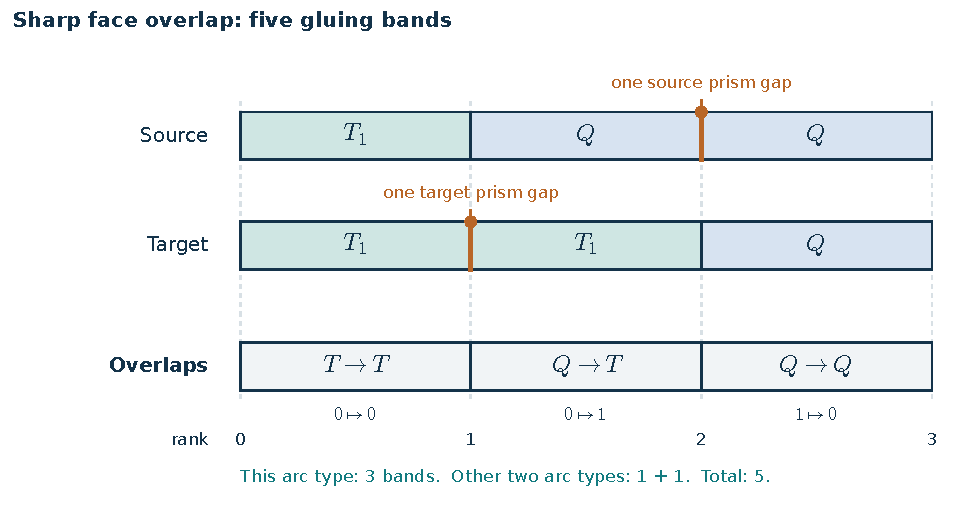
\includegraphics[width=\linewidth]{figures/normal_face_overlap.pdf}
\caption{Sharp local extraction at cut vertex $1$. The source blocks
$[0,1)$ and $[1,3)$ and target blocks $[0,2)$ and $[2,3)$ yield three
pairings. The two other arc types contribute one each, attaining five
bands. Orange marks locate the two singleton prism gaps meeting opposite
residual cells. The lower indices refer to the individual disc stacks.}
\label{fig:normal-face}
\end{figure}

These are local cut data. Around a triangulation edge, one must still
assemble and regularize the incident pieces, reconstruct boundary-pattern
attachments, and identify whole parallelity bundles. The output is not a
claim that the residual-cell labels already form a valid global handle
structure. In particular it is not an implementation of the full
compressed-cut theorem in Lackenby's hierarchy machinery.

\subsection{An explicit interface to interval orbit counting}

Let $n_s$ be the multiplicity of stack $s$, let
$o_s=\sum_{r<s}n_r$, and let $D=\sum_s n_s$.
Concatenate the disc intervals into $[0,D)$. A pairing
$i\mapsto\varepsilon i+c$ from stack $s$ to stack $u$ becomes
\[
 z\longmapsto\varepsilon z+(o_u+c-\varepsilon o_s)
 \quad\hbox{on }[o_s+a,o_s+b).
\]
This conversion is implemented as \texttt{orbit\_input}. Its orbits are
exactly the connected components of the normal surface: a path between
polygon interiors can be moved away from the finite set of polygon
vertices and then crosses a sequence of glued polygon sides. The algorithm
of Agol, Hass, and Thurston~\cite{aht} is the established polynomial-time method for
counting such interval orbits; the new code prepares its input but does
not implement that orbit-reduction algorithm.

The stored cyclic polygon orientations also give a signed version of
each side pairing. If the pairing preserves the two induced boundary
directions, consistent polygon-interior orientations differ by a minus
sign; if it reverses them, the interiors carry the same sign.
The implementation prepares the orientation double cover by making two
copies of every disc and switching copies exactly on negative transports.
If $C$ is the original orbit count and $\widetilde C$ the count in this
double cover, then
\[
 \#\{\text{orientable components}\}=\widetilde C-C,
 \qquad
 \#\{\text{nonorientable components}\}=2C-\widetilde C.
\]
Each orientable component contributes two cover components and each
nonorientable component contributes one. This is an aggregate count;
obtaining the full coordinate vector and topology of each compressed
component requires the weighted orbit machinery or an equally precise
replacement.

\subsection{Validation and measured scope}

The exact geometric oracle realizes triangle slices by
$z_v=1-(j+1)/(4(n+1))$ and quadrilateral slices by
$\sum_{a\in A}z_a=2/3-(j+1)/(3(n+1))$. It explicitly sorts the resulting
face arcs using rational numbers, independently of the block-overlay code.
The suite covers all 24 tetrahedral vertex permutations, four source faces,
and all choices of absent or active quadrilateral type on both sides,
with fixed-seed small multiplicities. It includes 1537 cases, the sharp
example above, and 591 reflected prism bands.

A separate comparison uses Regina~\cite{regina} on 807 small normal-surface inputs.
It compares full component coordinate multisets, Euler characteristics,
orientability, and boundary counts. This includes 92 nonorientable and
274 closed components, scalar multiples of one-sided surfaces, and compatible
normal sums that need not lie on extreme rays. Both interval-orbit adapters
are also checked by explicit finite equivalence relations. Large-coordinate
experiments run only the compressed extractor; neither the reference
expansion nor Regina's component routine is invoked there.

For the previously supplied Fibonacci meridian family at $t=128$, the
input encodes about $2.79\times10^{27}$ normal discs. The extractor returns
764 surface bands, 754 prism bands, 254 prism-to-residue contacts, and
512 local residual cells. At $t=1024$ it returns 6140 surface bands
and 4096 residual cells. Fixed-size tests with two tetrahedra and
65536-bit multiplicities retain ten stacks and four surface bands.
These measurements demonstrate a representation and extraction improvement;
they do not measure a complete unknot-recognition pipeline.
